% Options for packages loaded elsewhere
\PassOptionsToPackage{unicode}{hyperref}
\PassOptionsToPackage{hyphens}{url}
\PassOptionsToPackage{dvipsnames,svgnames,x11names}{xcolor}
%
\documentclass[
  letterpaper,
  DIV=11,
  numbers=noendperiod]{scrartcl}

\usepackage{amsmath,amssymb}
\usepackage{iftex}
\ifPDFTeX
  \usepackage[T1]{fontenc}
  \usepackage[utf8]{inputenc}
  \usepackage{textcomp} % provide euro and other symbols
\else % if luatex or xetex
  \usepackage{unicode-math}
  \defaultfontfeatures{Scale=MatchLowercase}
  \defaultfontfeatures[\rmfamily]{Ligatures=TeX,Scale=1}
\fi
\usepackage{lmodern}
\ifPDFTeX\else  
    % xetex/luatex font selection
\fi
% Use upquote if available, for straight quotes in verbatim environments
\IfFileExists{upquote.sty}{\usepackage{upquote}}{}
\IfFileExists{microtype.sty}{% use microtype if available
  \usepackage[]{microtype}
  \UseMicrotypeSet[protrusion]{basicmath} % disable protrusion for tt fonts
}{}
\makeatletter
\@ifundefined{KOMAClassName}{% if non-KOMA class
  \IfFileExists{parskip.sty}{%
    \usepackage{parskip}
  }{% else
    \setlength{\parindent}{0pt}
    \setlength{\parskip}{6pt plus 2pt minus 1pt}}
}{% if KOMA class
  \KOMAoptions{parskip=half}}
\makeatother
\usepackage{xcolor}
\setlength{\emergencystretch}{3em} % prevent overfull lines
\setcounter{secnumdepth}{-\maxdimen} % remove section numbering
% Make \paragraph and \subparagraph free-standing
\makeatletter
\ifx\paragraph\undefined\else
  \let\oldparagraph\paragraph
  \renewcommand{\paragraph}{
    \@ifstar
      \xxxParagraphStar
      \xxxParagraphNoStar
  }
  \newcommand{\xxxParagraphStar}[1]{\oldparagraph*{#1}\mbox{}}
  \newcommand{\xxxParagraphNoStar}[1]{\oldparagraph{#1}\mbox{}}
\fi
\ifx\subparagraph\undefined\else
  \let\oldsubparagraph\subparagraph
  \renewcommand{\subparagraph}{
    \@ifstar
      \xxxSubParagraphStar
      \xxxSubParagraphNoStar
  }
  \newcommand{\xxxSubParagraphStar}[1]{\oldsubparagraph*{#1}\mbox{}}
  \newcommand{\xxxSubParagraphNoStar}[1]{\oldsubparagraph{#1}\mbox{}}
\fi
\makeatother


\providecommand{\tightlist}{%
  \setlength{\itemsep}{0pt}\setlength{\parskip}{0pt}}\usepackage{longtable,booktabs,array}
\usepackage{calc} % for calculating minipage widths
% Correct order of tables after \paragraph or \subparagraph
\usepackage{etoolbox}
\makeatletter
\patchcmd\longtable{\par}{\if@noskipsec\mbox{}\fi\par}{}{}
\makeatother
% Allow footnotes in longtable head/foot
\IfFileExists{footnotehyper.sty}{\usepackage{footnotehyper}}{\usepackage{footnote}}
\makesavenoteenv{longtable}
\usepackage{graphicx}
\makeatletter
\def\maxwidth{\ifdim\Gin@nat@width>\linewidth\linewidth\else\Gin@nat@width\fi}
\def\maxheight{\ifdim\Gin@nat@height>\textheight\textheight\else\Gin@nat@height\fi}
\makeatother
% Scale images if necessary, so that they will not overflow the page
% margins by default, and it is still possible to overwrite the defaults
% using explicit options in \includegraphics[width, height, ...]{}
\setkeys{Gin}{width=\maxwidth,height=\maxheight,keepaspectratio}
% Set default figure placement to htbp
\makeatletter
\def\fps@figure{htbp}
\makeatother

\usepackage{sidecap}
\KOMAoption{captions}{tableheading}
\makeatletter
\@ifpackageloaded{caption}{}{\usepackage{caption}}
\AtBeginDocument{%
\ifdefined\contentsname
  \renewcommand*\contentsname{Table of contents}
\else
  \newcommand\contentsname{Table of contents}
\fi
\ifdefined\listfigurename
  \renewcommand*\listfigurename{List of Figures}
\else
  \newcommand\listfigurename{List of Figures}
\fi
\ifdefined\listtablename
  \renewcommand*\listtablename{List of Tables}
\else
  \newcommand\listtablename{List of Tables}
\fi
\ifdefined\figurename
  \renewcommand*\figurename{Figure}
\else
  \newcommand\figurename{Figure}
\fi
\ifdefined\tablename
  \renewcommand*\tablename{Table}
\else
  \newcommand\tablename{Table}
\fi
}
\@ifpackageloaded{float}{}{\usepackage{float}}
\floatstyle{ruled}
\@ifundefined{c@chapter}{\newfloat{codelisting}{h}{lop}}{\newfloat{codelisting}{h}{lop}[chapter]}
\floatname{codelisting}{Listing}
\newcommand*\listoflistings{\listof{codelisting}{List of Listings}}
\makeatother
\makeatletter
\makeatother
\makeatletter
\@ifpackageloaded{caption}{}{\usepackage{caption}}
\@ifpackageloaded{subcaption}{}{\usepackage{subcaption}}
\makeatother

\ifLuaTeX
  \usepackage{selnolig}  % disable illegal ligatures
\fi
\usepackage[]{natbib}
\bibliographystyle{plainnat}
\usepackage{bookmark}

\IfFileExists{xurl.sty}{\usepackage{xurl}}{} % add URL line breaks if available
\urlstyle{same} % disable monospaced font for URLs
\hypersetup{
  pdftitle={Exploring solar wind discontinuity properties in the inner and outer heliosphere},
  colorlinks=true,
  linkcolor={blue},
  filecolor={Maroon},
  citecolor={Blue},
  urlcolor={Blue},
  pdfcreator={LaTeX via pandoc}}


\title{Exploring solar wind discontinuity properties in the inner and outer heliosphere}
\author{}
\date{}

\begin{document}
\maketitle

\vspace{-20truemm}


\textbf{PhD Candidate: Zijin Zhang}

\subsection{Abstract}\label{abstract}

Solar wind discontinuities, characterized by abrupt changes in the magnetic field, play a crucial role in heliospheric dynamics, such as solar wind heating and turbulence. This proposal aims to conduct a detailed study of these discontinuities, leveraging data from contemporary space missions like Parker Solar Probe (PSP) and Juno to examine their characteristics (occurrence rates, thickness, current density and Alfvenicity, etc.) from the Sun to beyond 1 AU. By analyzing the evolution of these features, this study seeks to answer questions about how the discontinuities change with the radial distance from the Sun and the physical mechanisms behind the formation of solar wind discontinuities.

\subsection{Introduction and Background}\label{introduction-and-background}

The study of solar wind magnetic discontinuities, characterized by rapid variations in interplanetary magnetic fields, stands at the forefront of understanding key phenomena in Heliophysics. These discontinuities, manifesting as localized transient rotations or jumps in the magnetic field, are pivotal in processes such as efficient plasma heating and in hosting plasma instabilities associated with discontinuity currents, which are among the most intense currents in the solar wind. Theoretical models suggest that the formation and destruction of discontinuities are closely related to the nonlinear dynamics of Alfvén waves. These nonlinear processes can create significant isolated disturbances to the otherwise adiabatic evolution of the solar wind flow. Investigatation of the nonfluid (kinetic) properties of solar wind discontinuities reveals that electron density and temperature vary significantly across these discontinuities, underlining the importance of kinetic effects in discontinuity structure.

As such, this study aims to understand the dynamics of solar wind discontinuities by addressing the key question

\textbf{``How do discontinuities evolve over radial distances from the Sun and what are the physical mechanisms behind their formation and evolution?''}

Understanding these discontinuities is essential for elucidating the fundamental processes that govern the solar wind's evolution as it travels through the heliosphere.

\subsubsection{Previous Studies and Context}\label{previous-studies-and-context}

Spacecraft investigations of the space plasma environment have revealed that the solar wind magnetic field follows the Parker model of the heliospheric current sheet only on average. Localized transient currents, that can be significantly more intense than the model currents, are carried by various discontinuities observed as strong variations in magnetic field components \citep{colburnDiscontinuitiesSolarWind1966, burlagaMicroscaleStructuresInterplanetary1968, turnerOrientationsRotationalTangential1971}. Most often such variations are manifested as magnetic fieild rotations within the plane of two most fluctuating components.

Further advancements were made with data from the Helios-1, Helios-2, Ulysses and Voyager missions, which explored discontinuities in three-dimensional space, revealing their prevalence and importance throughout the heliosphere \citep{marianiStatisticalStudyMagnetohydrodynamic1983, tsurutaniNonlinearElectromagneticWaves1997}. As illustrated in Figure~\ref{fig-1}, these discontinuities are observed at a multitude of radial distances from the Sun. These findings underscored the need to understand the origin of discontinuities, which are thought to arise from dynamic processes on the Sun, including solar flares and coronal mass ejections, as well as through in-situ processes like local magnetic turbulence, magnetic reconnection and nonlinear wave interactions within the solar wind.

\begin{figure}

\centering{

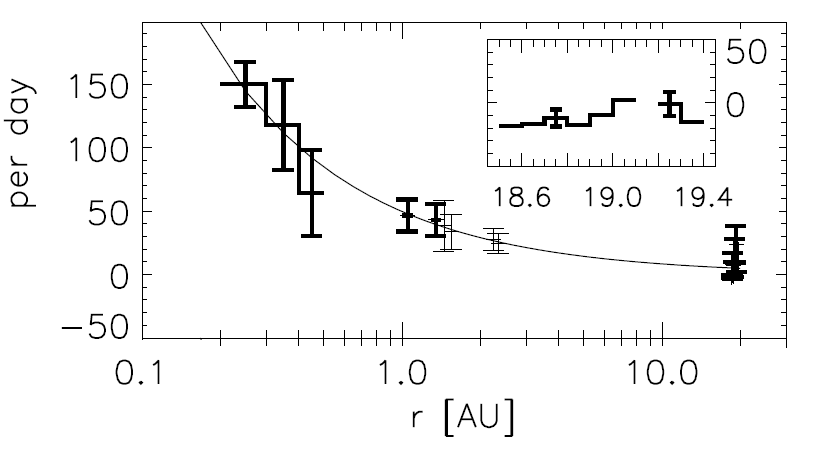
\includegraphics[width=0.75\textwidth,height=\textheight]{figures/schematic.png}

}

\caption{\label{fig-1}Distribution of occurrence rate of solar wind discontinuities \citep{sodingRadialLatitudinalDependencies2001}.}

\end{figure}%

\subsubsection{The Role of Alfven wave and kinetic effects in the discontinuities}\label{the-role-of-alfven-wave-and-kinetic-effects-in-the-discontinuities}

Ulysses measurements of the high-latitude solar wind at \(1-5\) AU showed that the majority of discontinuities resided within the stream-stream interaction regions and/or within Alfvén wave trains \citep{tsurutaniInterplanetaryDiscontinuitiesAlfven1995, tsurutaniReviewDiscontinuitiesAlfven1999}. The nonlinear evolution of Alfvén waves (wave steepening) can be the main cause of such discontinuities. The background plasma/magnetic field inhomogeneities and various dissipative processes are key to Alfvén wave nonlinear evolution \citep{Lerche75, Prakash&Diamond99, Medvedev97:prl, Nariyuki14, Yang15}. In hybrid simulations \citep[see][]{Vasquez&Hollweg98, Vasquez&Hollweg01, TenBarge&Howes13} and analytical models \citep[e.g.,][]{Kennel88:jetp, Hada89, Malkov91, Wu&Kennel92, Medvedev97:pop}, this steepening was shown to cause formation of discontinuities in configurations resembling the near-Earth observations. There are models predicting discontinuity formation \citep{Servidio15, Podesta&Roytershteyn17} and destruction \citep{Servidio11,Matthaeus15} due to dissipative processes (e.g., Alfvén wave steepening, magnetic reconnection) in the solar wind. However, the efficiency of these processes in realistic expanding solar wind was not yet tested against observations.

More recently, utilizing high-resolution plasma measurements from ARTEMIS and MMS missions, \citet{artemyevKineticNatureSolar2019} showed that discontinuities have kinetic characteristics for both tangential and rotational discontinuities: fluxes of electrons of different energies vary differently across these discontinuities. This discoveries revealed the importance of ion and electron kinetics to discontinuity structure.

\subsubsection{Current Gaps in Understanding}\label{current-gaps-in-understanding}

Previous observations of solar wind discontinuities in the outer heliosphere were rarely in conjunction with measurements closer to the Sun. Thus it is presently unclear whether the observed changes in their frequency and properties are due to variations in the solar plasma state resulting from solar variability, such as the solar magnetic activity cycle, or whether these changes are a natural outcome of the discontinuities' propagation and interaction with the ambient solar wind.

Regular and long-lasting Juno (2011-2016) and PSP (2019-now) observations together with almost permanent near-Earth solar wind monitoring provide a unique opportunity to examine the discontinuity characteristics at two radial distances simultaneously in the context of both the inner and in the outer heliosphere over an large radial distance range (\(\sim 0.1\) AU - \(\sim 5\) AU). We will determine the discontinuity occurrence rates and properties for various radial distances and compare these results with the prediction of the adiabatic expansion model, \textbf{to understand if discontinuity formation or destruction dominate the statistics of discontinuities far away from the solar wind acceleration region}.

This research seeks to address these gaps by leveraging recent advancements in observational capabilities and numerical modeling to provide a comprehensive examination of solar wind discontinuities.

\subsection{Methodology}\label{methodology}

\textbf{Data Collection and Model:}

\textbf{Parker Solar Probe} and \textbf{Juno} provide high-resolution magnetic field and plasma data from the inner heliosphere to beyond 1 AU. The PSP's close passes to the Sun offer unique insights into the nascent solar wind, while Juno's trajectory up to Jupiter allows for studying the evolution of solar wind structures as they propagate outward.

The solar wind plasma state, as evidenced by the sunspot number (referenced in Figure~\ref{fig-overview}), plays a crucial role in understanding the dynamics of discontinuities. During the initial phase of the JUNO mission, the sunspot number reached its peak, indicating a period of heightened solar activity. However, by the end of the mission's cruise phase, there was a significant decline in solar activity. This variation underscores the importance of calibrating the discontinuity properties in relation to solar activity levels to account for temporal fluctuations.

Further analysis of Figure~\ref{fig-overview} highlights the significance of the heliographic longitudinal difference between the Juno mission and Earth as well as the STEREO-A mission. Specifically, when there is a substantial longitudinal difference between Juno and Earth, the difference between Juno and STEREO-A tends to be minimal, and vice versa. This longitudinal discrepancy between Earth and STEREO-A ensures comprehensive coverage of the plasma en route to Juno.

\begin{figure}

\centering{

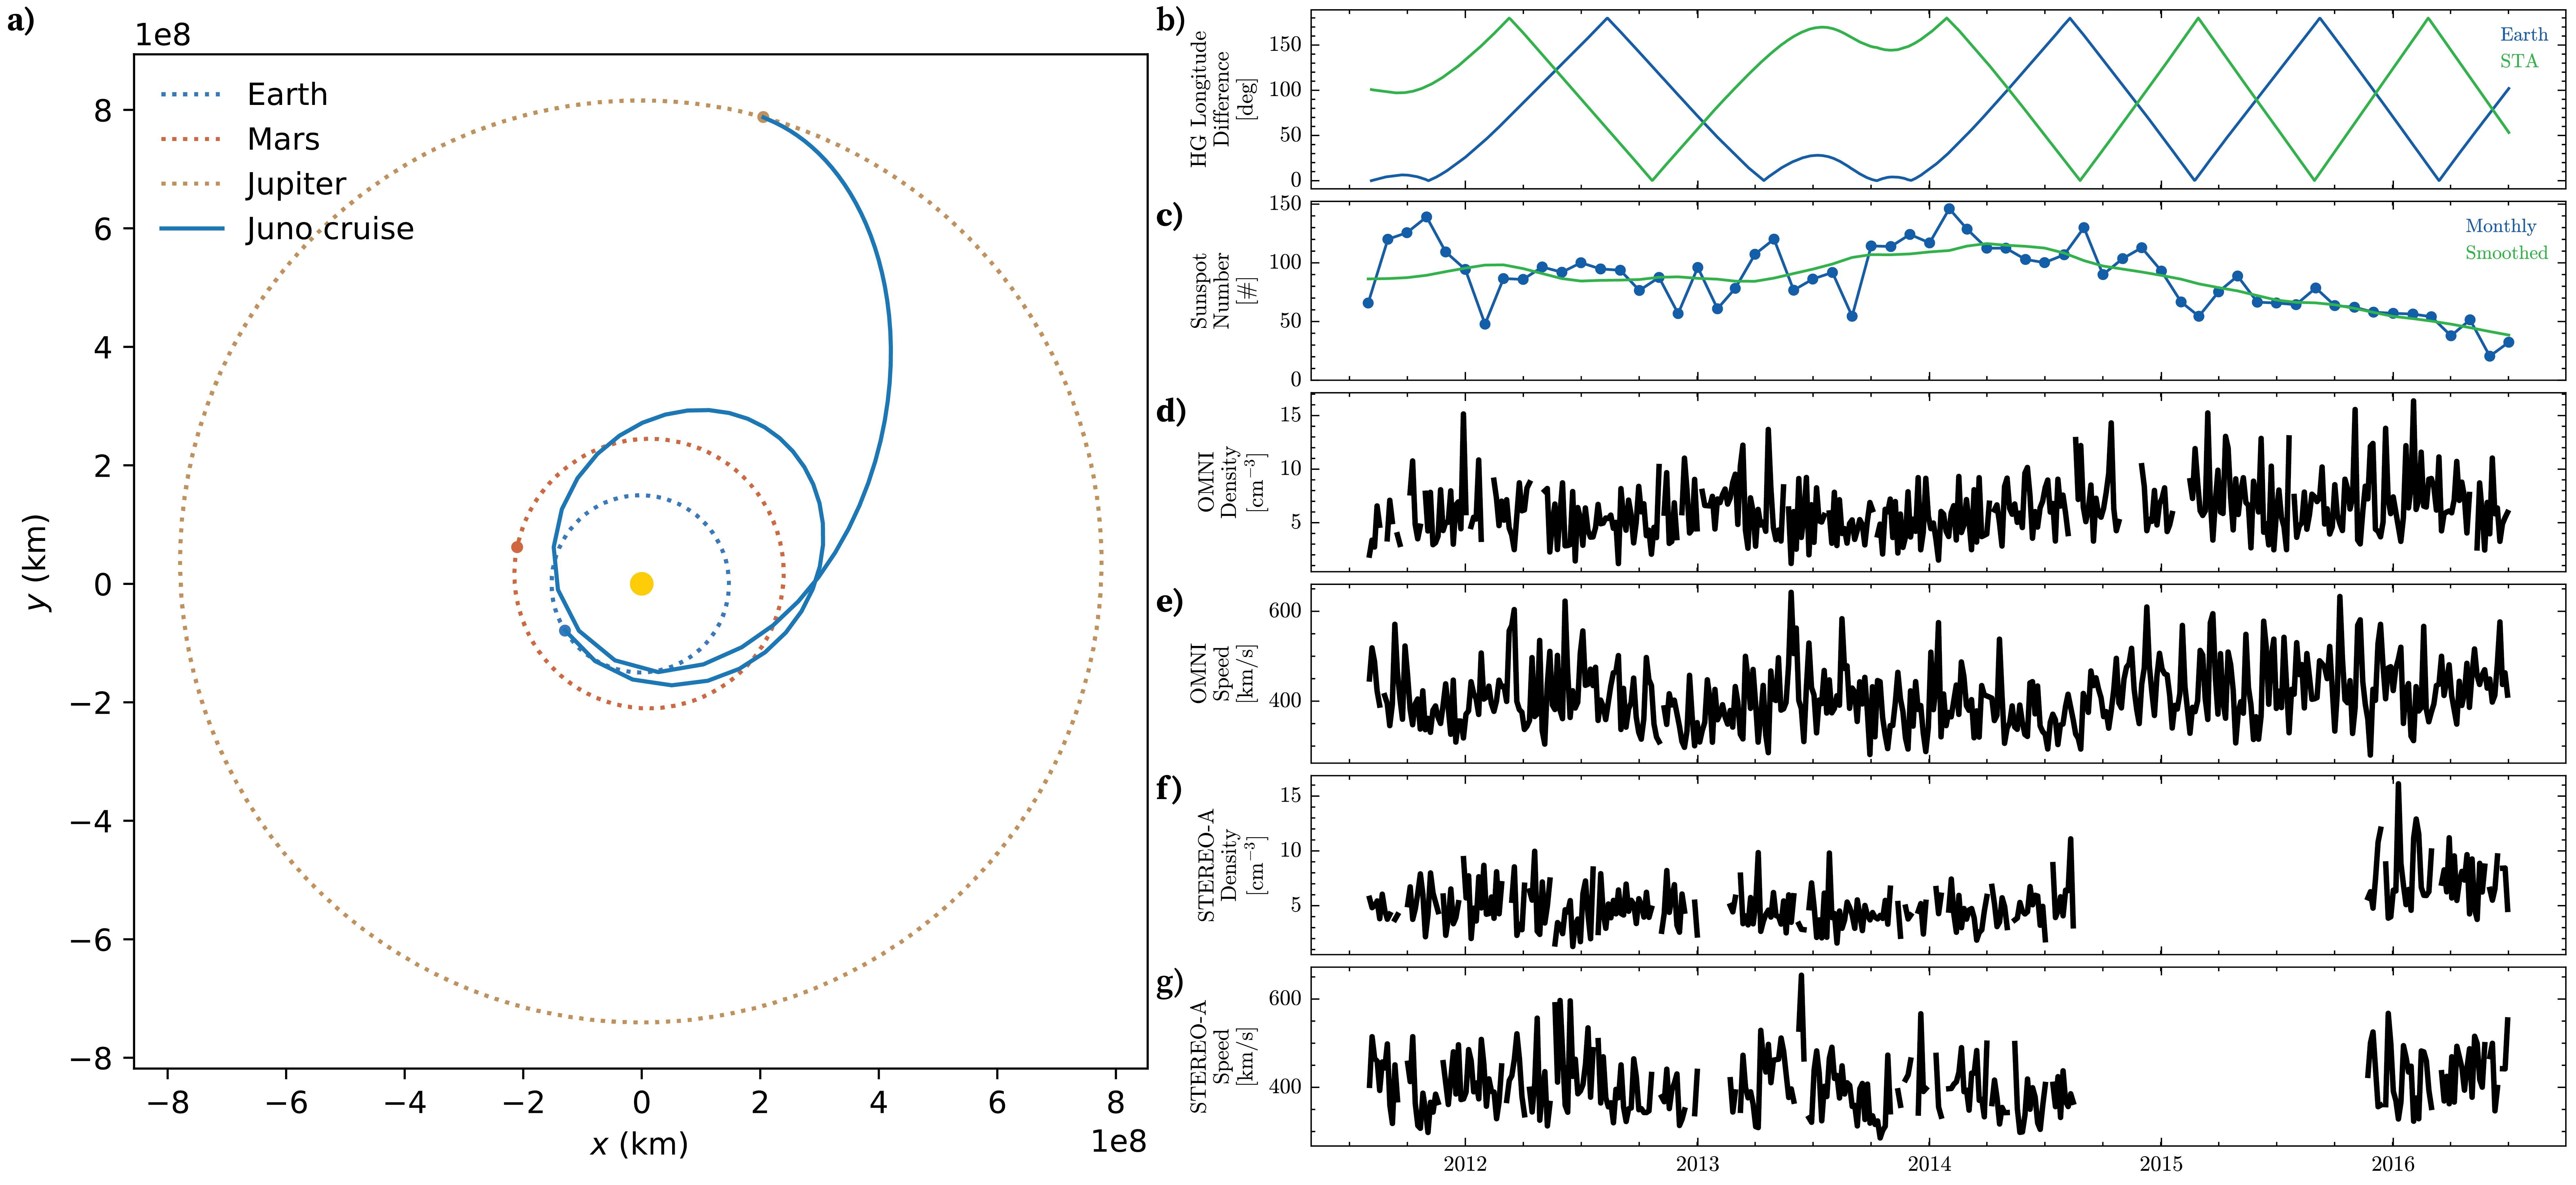
\includegraphics{figures/fig_overview.png}

}

\caption{\label{fig-overview}Overview. \textbf{a,} Juno orbit during its cruise phase (2011-2016). \textbf{b,} Difference of heliographic longitude of Juno and 1-AU missions. \textbf{c,} monthly and smoothed sunspot number. \textbf{d-g,} Near-Earth (OMNI) and STEREO-A solar wind plasma density and speed.}

\end{figure}%

Datasets from missions such as STEREO, ARTEMIS, and WIND will complement observations from PSP and Juno, offering a broader contextual perspective on heliospheric conditions and enabling a multi-point analysis of discontinuity properties \citep{velliUnderstandingOriginsHeliosphere2020}. The table below summarizes the time resolution of magnetic field and plasma data for PSP, Juno, Wind, ARTEMIS, and STEREO. However, since Juno does not provide direct plasma measurements, we will estimate the spatial scale (thickness) of discontinuities using solar wind speed derived from solar wind propagation models. Specifically, we will employ the Two-Dimensional Outer Heliosphere Solar Wind Modeling (MSWIM2D) \citep{keeblerMSWIM2DTwodimensionalOuter2022} to determine the ion bulk velocity (\(v\)) and plasma density (\(n\)) at Juno's location. This model, which utilizes the BATSRUS MHD solver, simulates the propagation of solar wind from 1 to 75 astronomical units (AU) in the ecliptic plane, effectively covering the region pertinent to our study. The MSWIM2D model provides output data with an hourly time resolution as shown in Figure~\ref{fig-model}. The comparison of magnetic field magnitudes from MSWIM2D with those measured by Juno, after averaging to the same time resolution, reveals a strong correlation, confirming the model's reliability.

\begin{longtable}[]{@{}lll@{}}
\toprule\noalign{}
Mission & δt(B) & δt(plasma) \\
\midrule\noalign{}
\endhead
\bottomrule\noalign{}
\endlastfoot
Parker Solar Probe & \textasciitilde200 Hz & 0.25-1 Hz \\
Juno & 1 Hz & 1 hour \\
ARTEMIS & 5 Hz & 0.25 Hz \\
WIND & 11 Hz & 1 Hz \\
STEREO & 8 Hz & 1 min \\
\end{longtable}

\textbf{Discontinuity Identification and Analysis:}

This first step in understanding the evolution of solar wind discontinuities involves identifying and characterizing these structures. We will adopt Liu's method \citep{liuMagneticDiscontinuitiesSolar2022} for this purpose, as it demonstrates better compatibility with discontinuities exhibiting minor field changes and is more robust to the situation encountered in the outer heliosphere.
Subsequently, for each identified discontinuity, we calculate the distance matrix of the time series sequence (the distance between each pair of magnetic field vectors) to ascertain its leading and trailing edges.
After that, we will utilize the minimum or maximum variance analysis (MVA) analysis \citep{sonnerupMinimumMaximumVariance1998, sonnerupMagnetopauseStructureAttitude1967} to determine the main (most varying) magnetic field component, \(B_l\), and medium variation component, \(B_m\).
The magnetic field component along the maximum variance direction is then fitted by a step-like functions to extract the parameters (we used logistic function here \(B(t; A, \mu, \sigma, {\mathrm{form=logistic}}) = A \left[1 - \frac{1}{1 + e^{\alpha}} \right]\), where \(\alpha = (t - \mu)/{\sigma}\)).
While previous studies \citep{vaskoKineticscaleCurrentSheets2021, vaskoKineticscaleCurrentSheets2022}, typically using data from a single spacecraft, often calculate current intensity by taking the derivative of the time series, our study must account for the varying time resolutions of different spacecraft. To address this, we fit the data to achieve a more precise representation of the peak current density, \(J_m = - \frac{1}{\mu_0 V_n} \frac{d B_m}{d t}\), thereby minimizing the impact of time resolution discrepancies.

Examples of solar wind discontinuities detected by various spacecraft are illustrated in Figure~\ref{fig-examples}.

\begin{figure}

\centering{

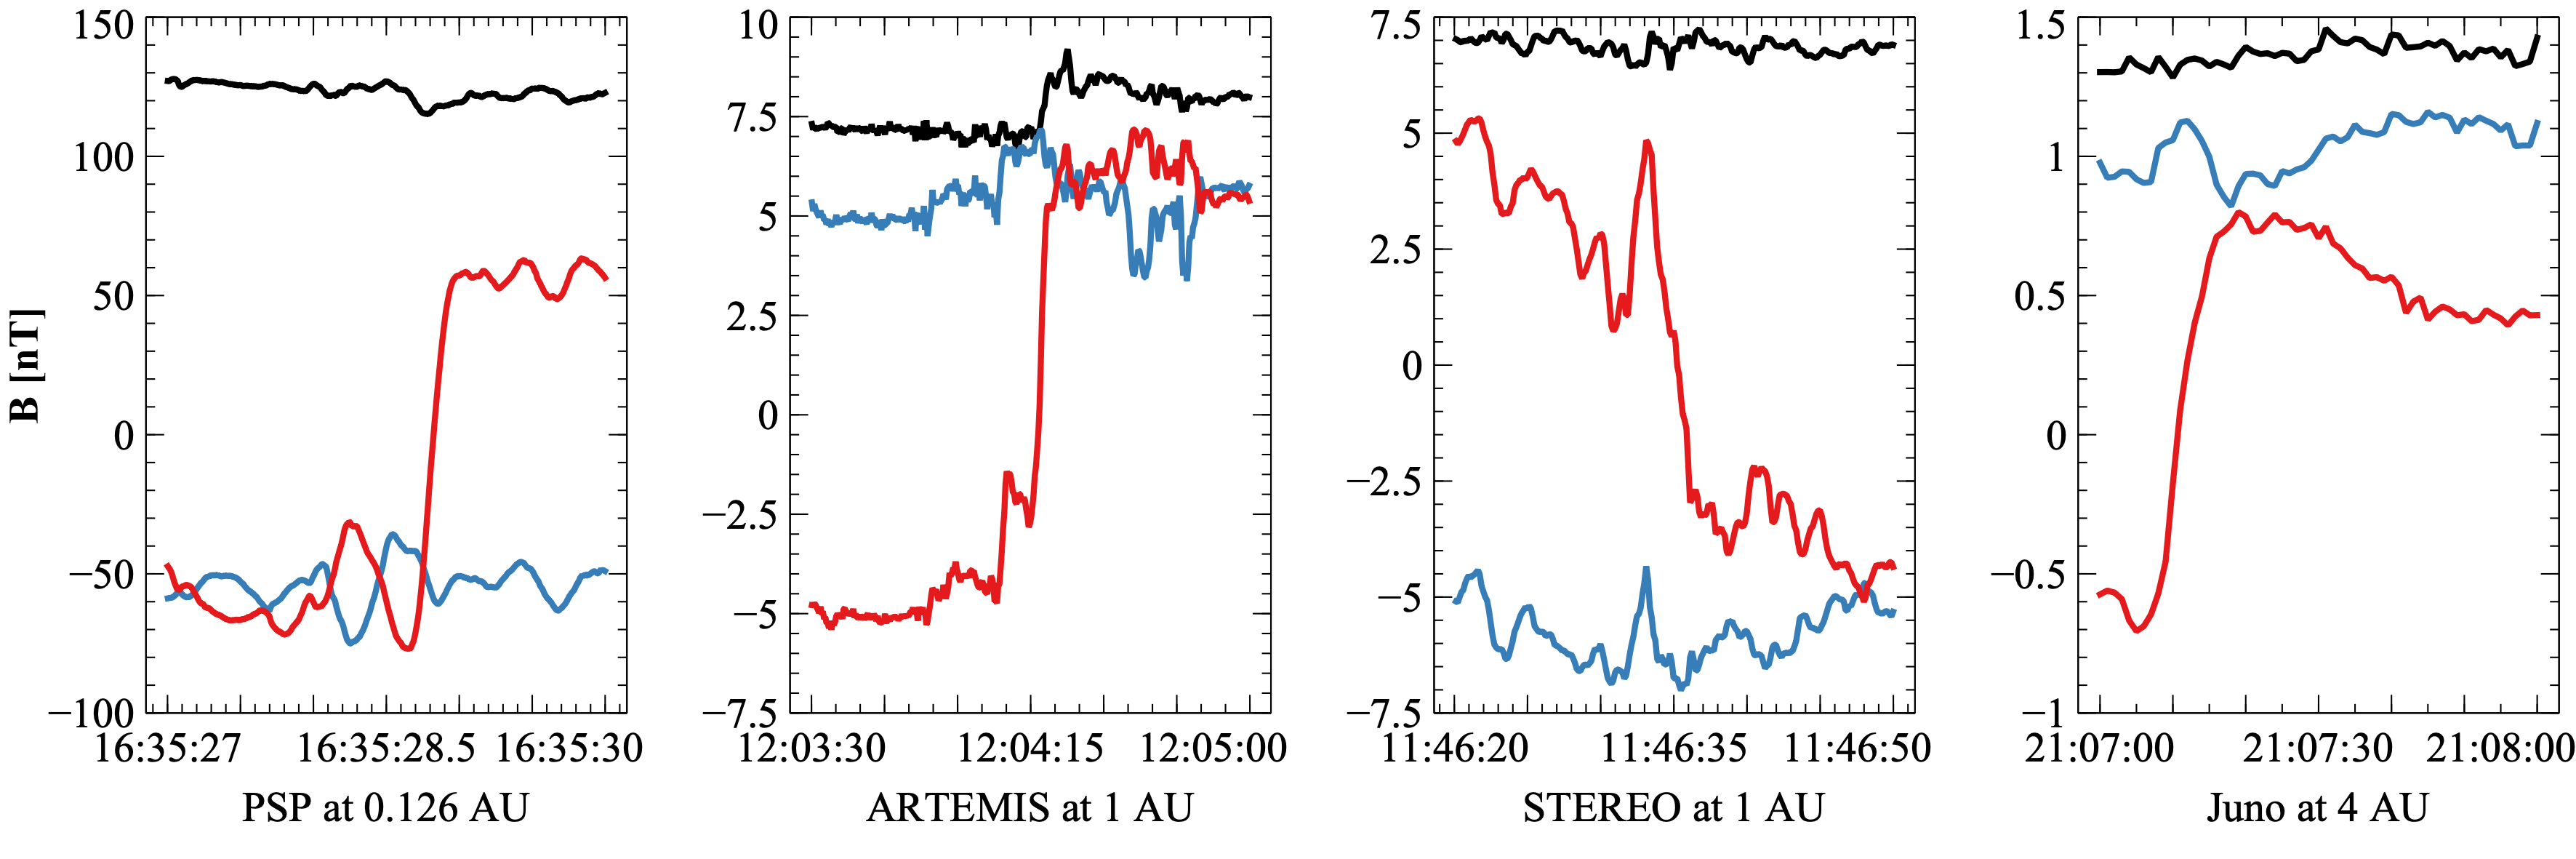
\includegraphics{figures/fig-ids_examples.png}

}

\caption{\label{fig-examples}Discontinuities detected by PSP, Juno, STEREO and near-Earth ARTEMIS satellite: red, blue, and black lines are \(B_l\), \(B_m\), and \(|{\mathbf B}|\).}

\end{figure}%

\textbf{Proposed Approach:}

Two promising approaches are proposed for studying the evolution of solar wind discontinuities:
\textbf{1. Conjunction Events Analysis:} This approach involves studying instances where spacecraft are either simultaneously aligned along the same spiral field line, thus measuring solar wind emanating from the same solar surface region, or positioned to measure the same solar wind plasma \citep{velliUnderstandingOriginsHeliosphere2020}. The latter alignment is determined by the difference in radial distance, \(\delta R\), corresponding to the solar wind travel time, \(\tau = \delta R / V_{sw}\).
An example demonstrating this approach is presented in Figure~\ref{fig-alignment}, showcasing similar trends in magnetic field magnitude, plasma density, velocity, and temperature observed by the Parker Solar Probe (PSP) and the Advanced Composition Explorer (ACE) during an alignment period in April 2019. Validation is further supported by utilizing the statistical plasma expansion model \citep{perroneRadialEvolutionSolar2019}, where the plasma properties measured by PSP and projected to the ACE location exhibit good agreement with actual ACE measurements, as depicted in Figure~\ref{fig-evolution}. This confirms the validity of the alignment approach for studying solar wind discontinuities.
\textbf{2. Comparative Analysis:} This approach leverages extensive data collected over the years to compare solar wind discontinuities observed by different spacecraft at various radial distances. Due to the Sun's rapid rotation, solar wind plasma emitted from a single region on the solar surface sweeps across the entire heliosphere within a solar rotation period of 27 days. By utilizing solar wind measurements at 1 AU from STEREO, ARTEMIS, and WIND, and comparing these with data from Juno and PSP, it is possible to distinguish between the effects of temporal variations in solar wind and those due to spatial variations (associated with radial distance from the Sun) in the occurrence rate and characteristics of discontinuities. An example of such a comparison for the occurrence rate is depicted in Figure~\ref{fig-rate}, where the number of discontinuities measured per day by different spacecraft missions is plotted.

\begin{figure}

\centering{

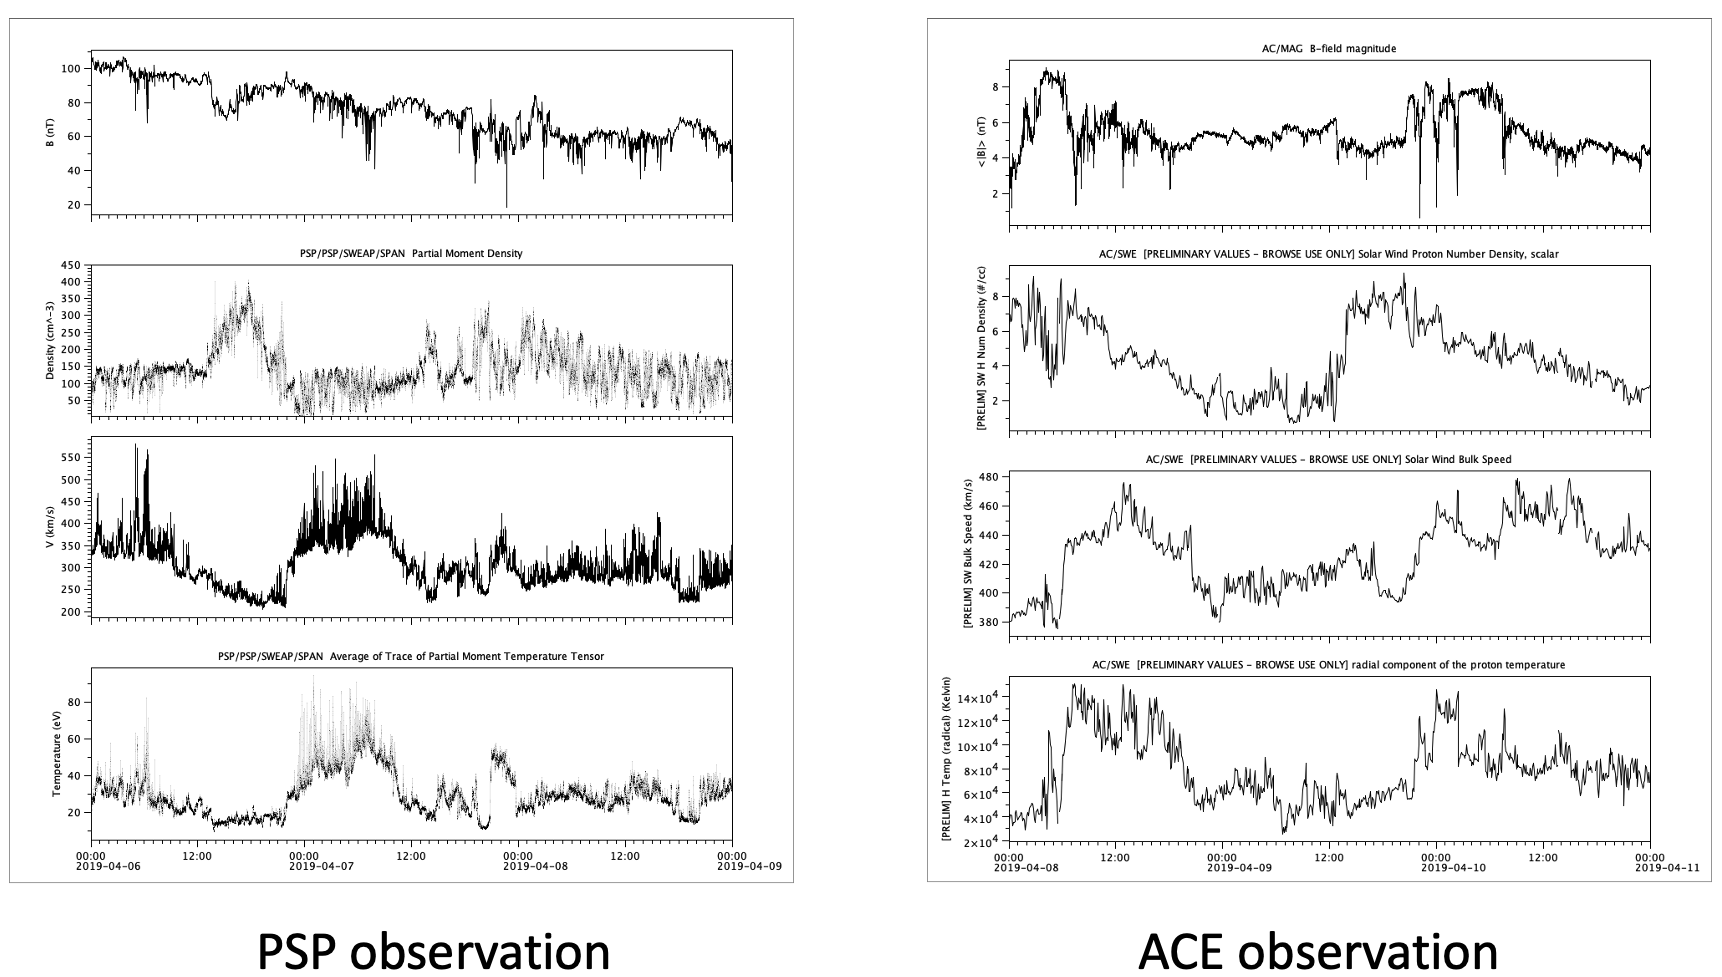
\includegraphics{figures/psp_alignment.png}

}

\caption{\label{fig-alignment}Measurement by PSP and ACE spacecrafts from 2019-04-06 to 2019-04-10. From top to bottom: (a) Magnetic field magnitude measured (b) Plasma density, (c) Plasma velocity, (d) Plasma temperature.}

\end{figure}%

In the proposed study, we will expand this comparison to include the properties of discontinuities, such as thickness, strength (current density), and orientation.

This extension will enable us to grasp how these features evolve with radial distance from the Sun and how they relate to the local plasma properties. Examining these properties is crucial for understanding the generation of discontinuities.
\citet{borovskyFluxTubeTexture2008} argued that solar wind discontinuities act as static boundaries between flux tubes originating at the solar surface and they are convected passively from the source regions. However, \citet{grecoStatisticalAnalysisDiscontinuities2009}, by examining the waiting time distribution of magnetic field increments, discovered a good agreement between between MHD simulations and observations. This finding suggests that discontinuities stem from intermittent MHD turbulence, indicating local generation.
If turbulence theory holds true, discontinuities properties should align with local plasma parameters; conversely, if propagation theory is accurate, discontinuities properties should be consistent with solar wind expansion model. Studying these properties will provide insights into the physical mechanisms governing discontinuity formation and spatial evolution as solar wind propagates through the heliosphere.

\begin{figure}

\centering{

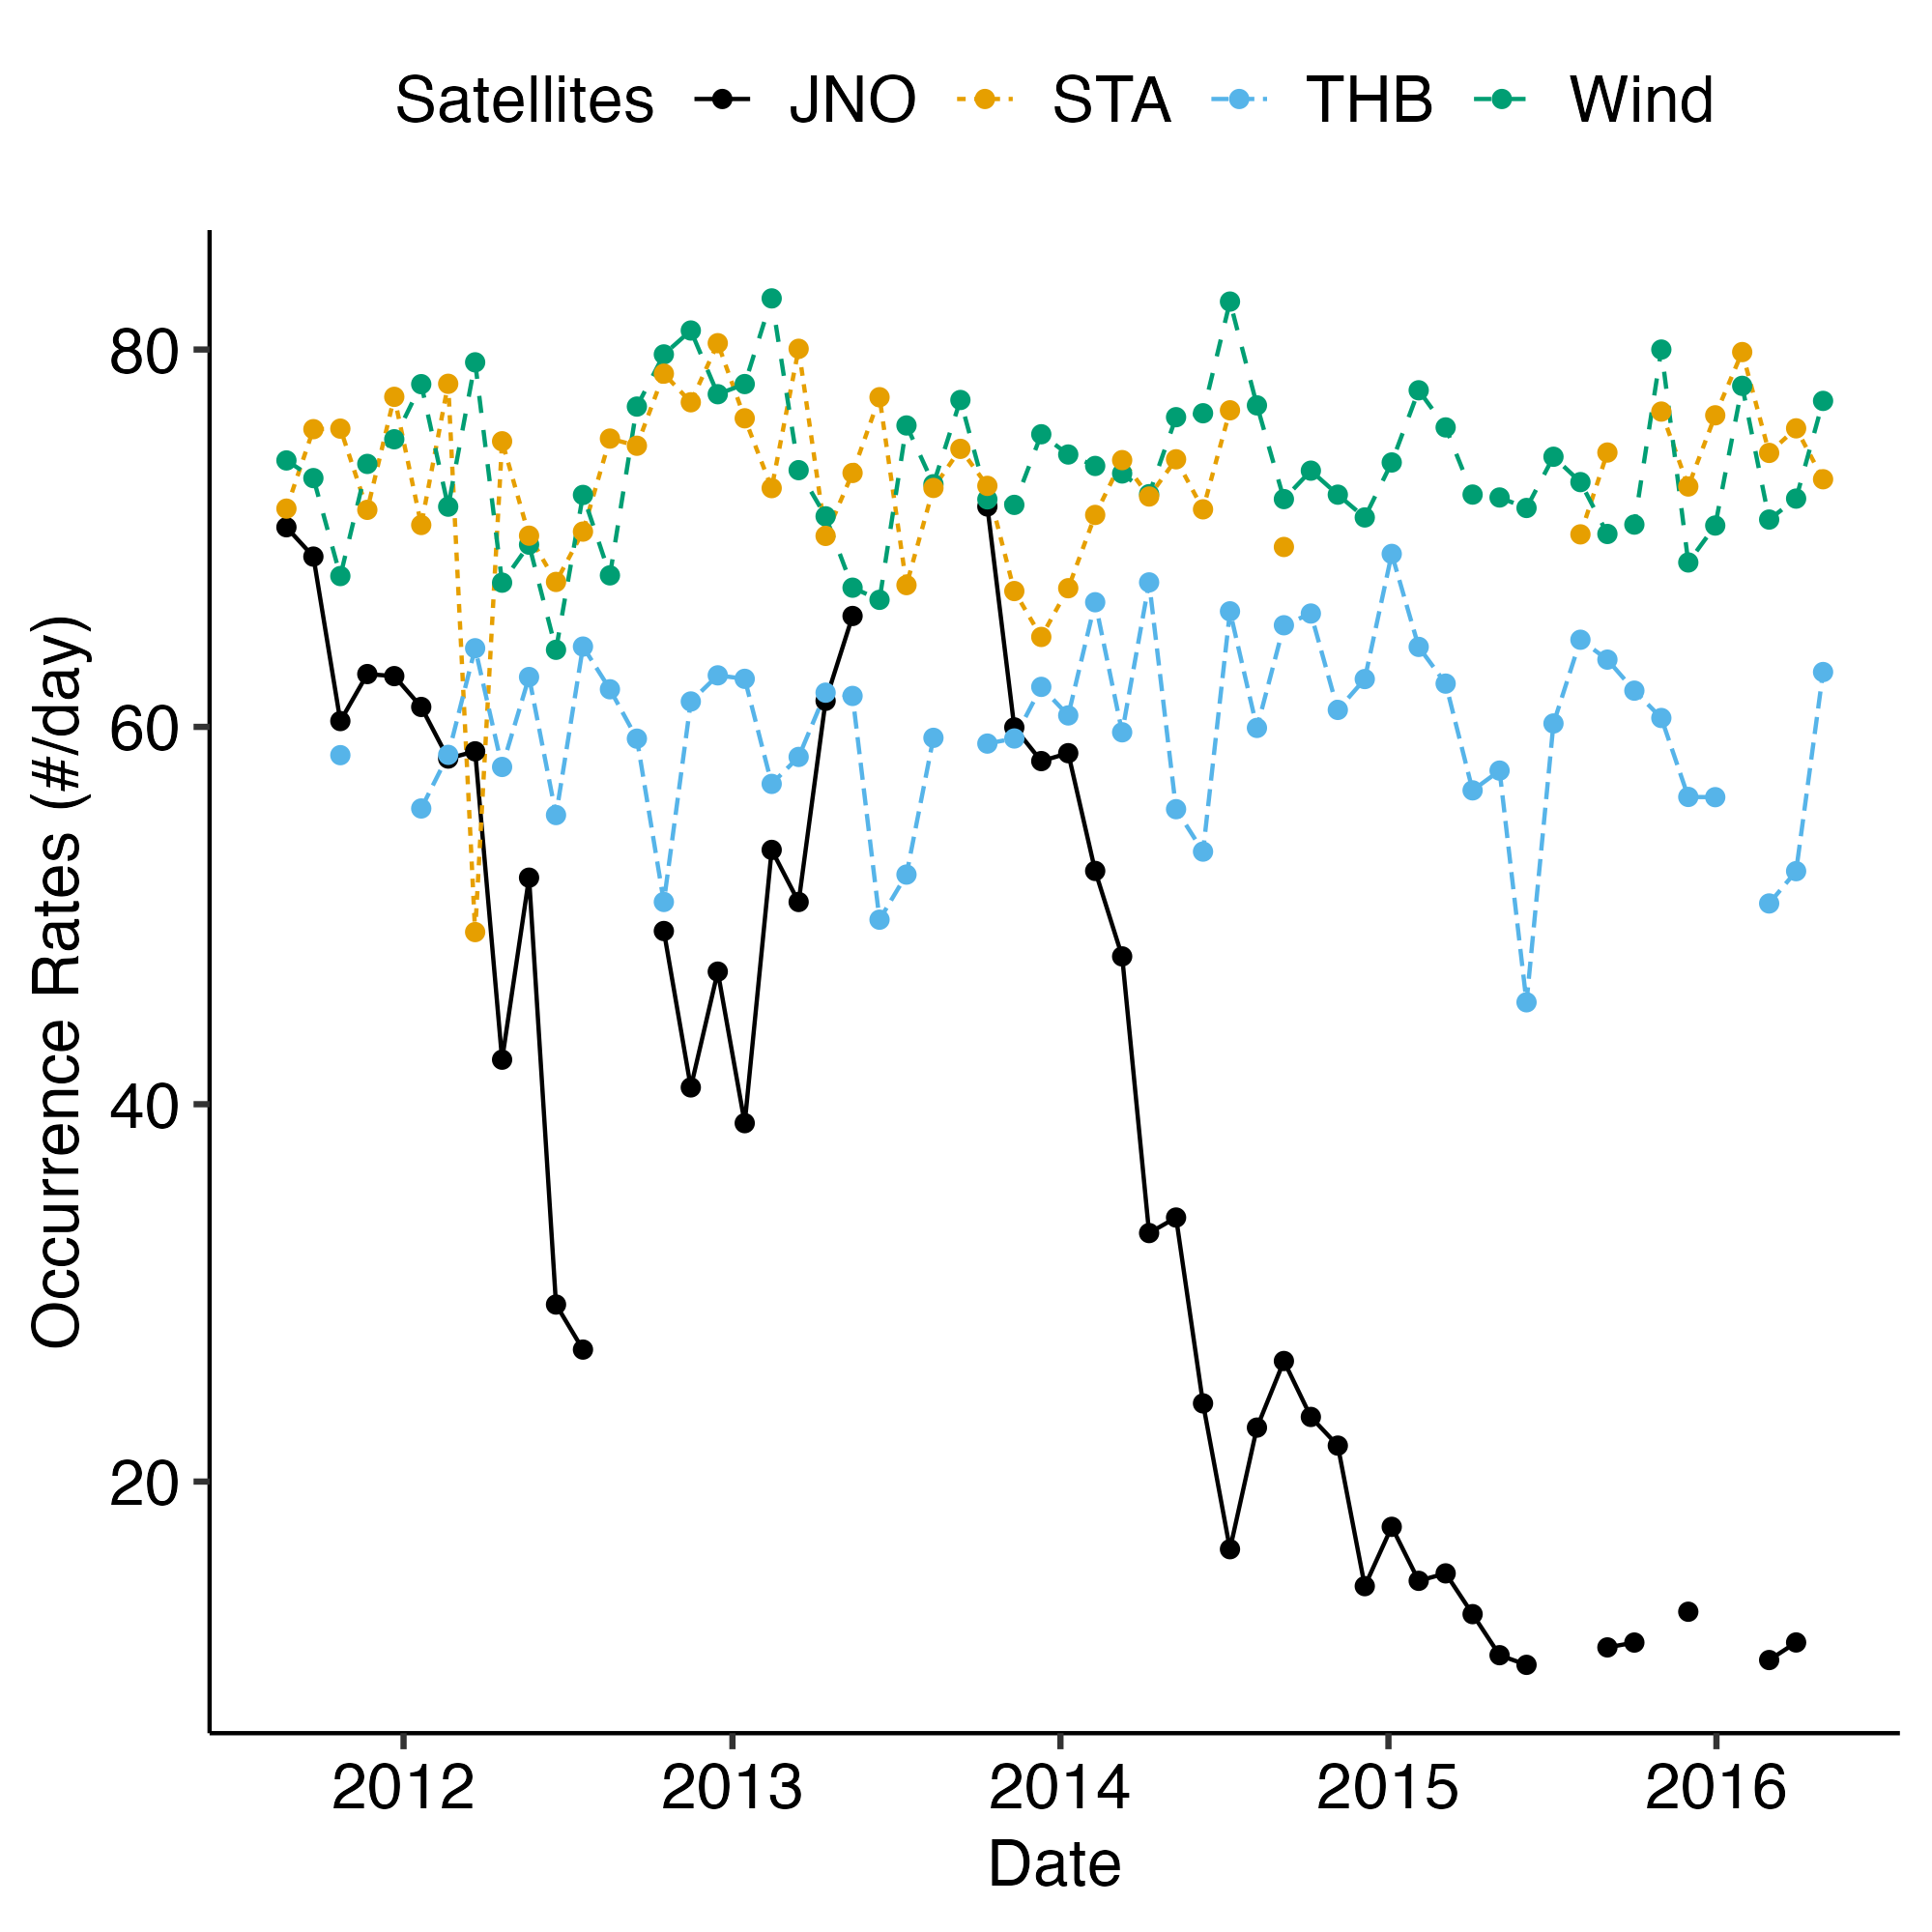
\includegraphics{figures/ocr_time_cleaned.png}

}

\caption{\label{fig-rate}The number of discontinuities measured by Juno per day coincides with the discontinuity number measured by STEREO, WIND, and ARTEMIS, when Juno is around \(1\) AU. This number (occurrence rate) decreases with distance (with time after \(\sim 2013\)), as Juno moves from \(1\) AU to \(5\) AU. We will use the similar comparison for discontinuity characteristics and occurrence rate derived for PSP and Juno.}

\end{figure}%

\subsection{Summary}\label{summary}

This research project adopts a comprehensive approach to unravel the complex characteristics of solar wind discontinuities, seeking to shed light on their fundamental characteristics. By utilizing big data from multiple spacecraft missions throughout the heliosphere, we aim to examine the temporal variations in these properties driven by solar activity, as well as the spatial variations influenced by radial distance from the Sun. Our goal is to infer the intricate processes governing the evolution of magnetic discontinuities, a key component of magnetic field turbulence and a crucial interface for charged particle acceleration.

\subsection{Figures}\label{figures}

\begin{figure}

\centering{

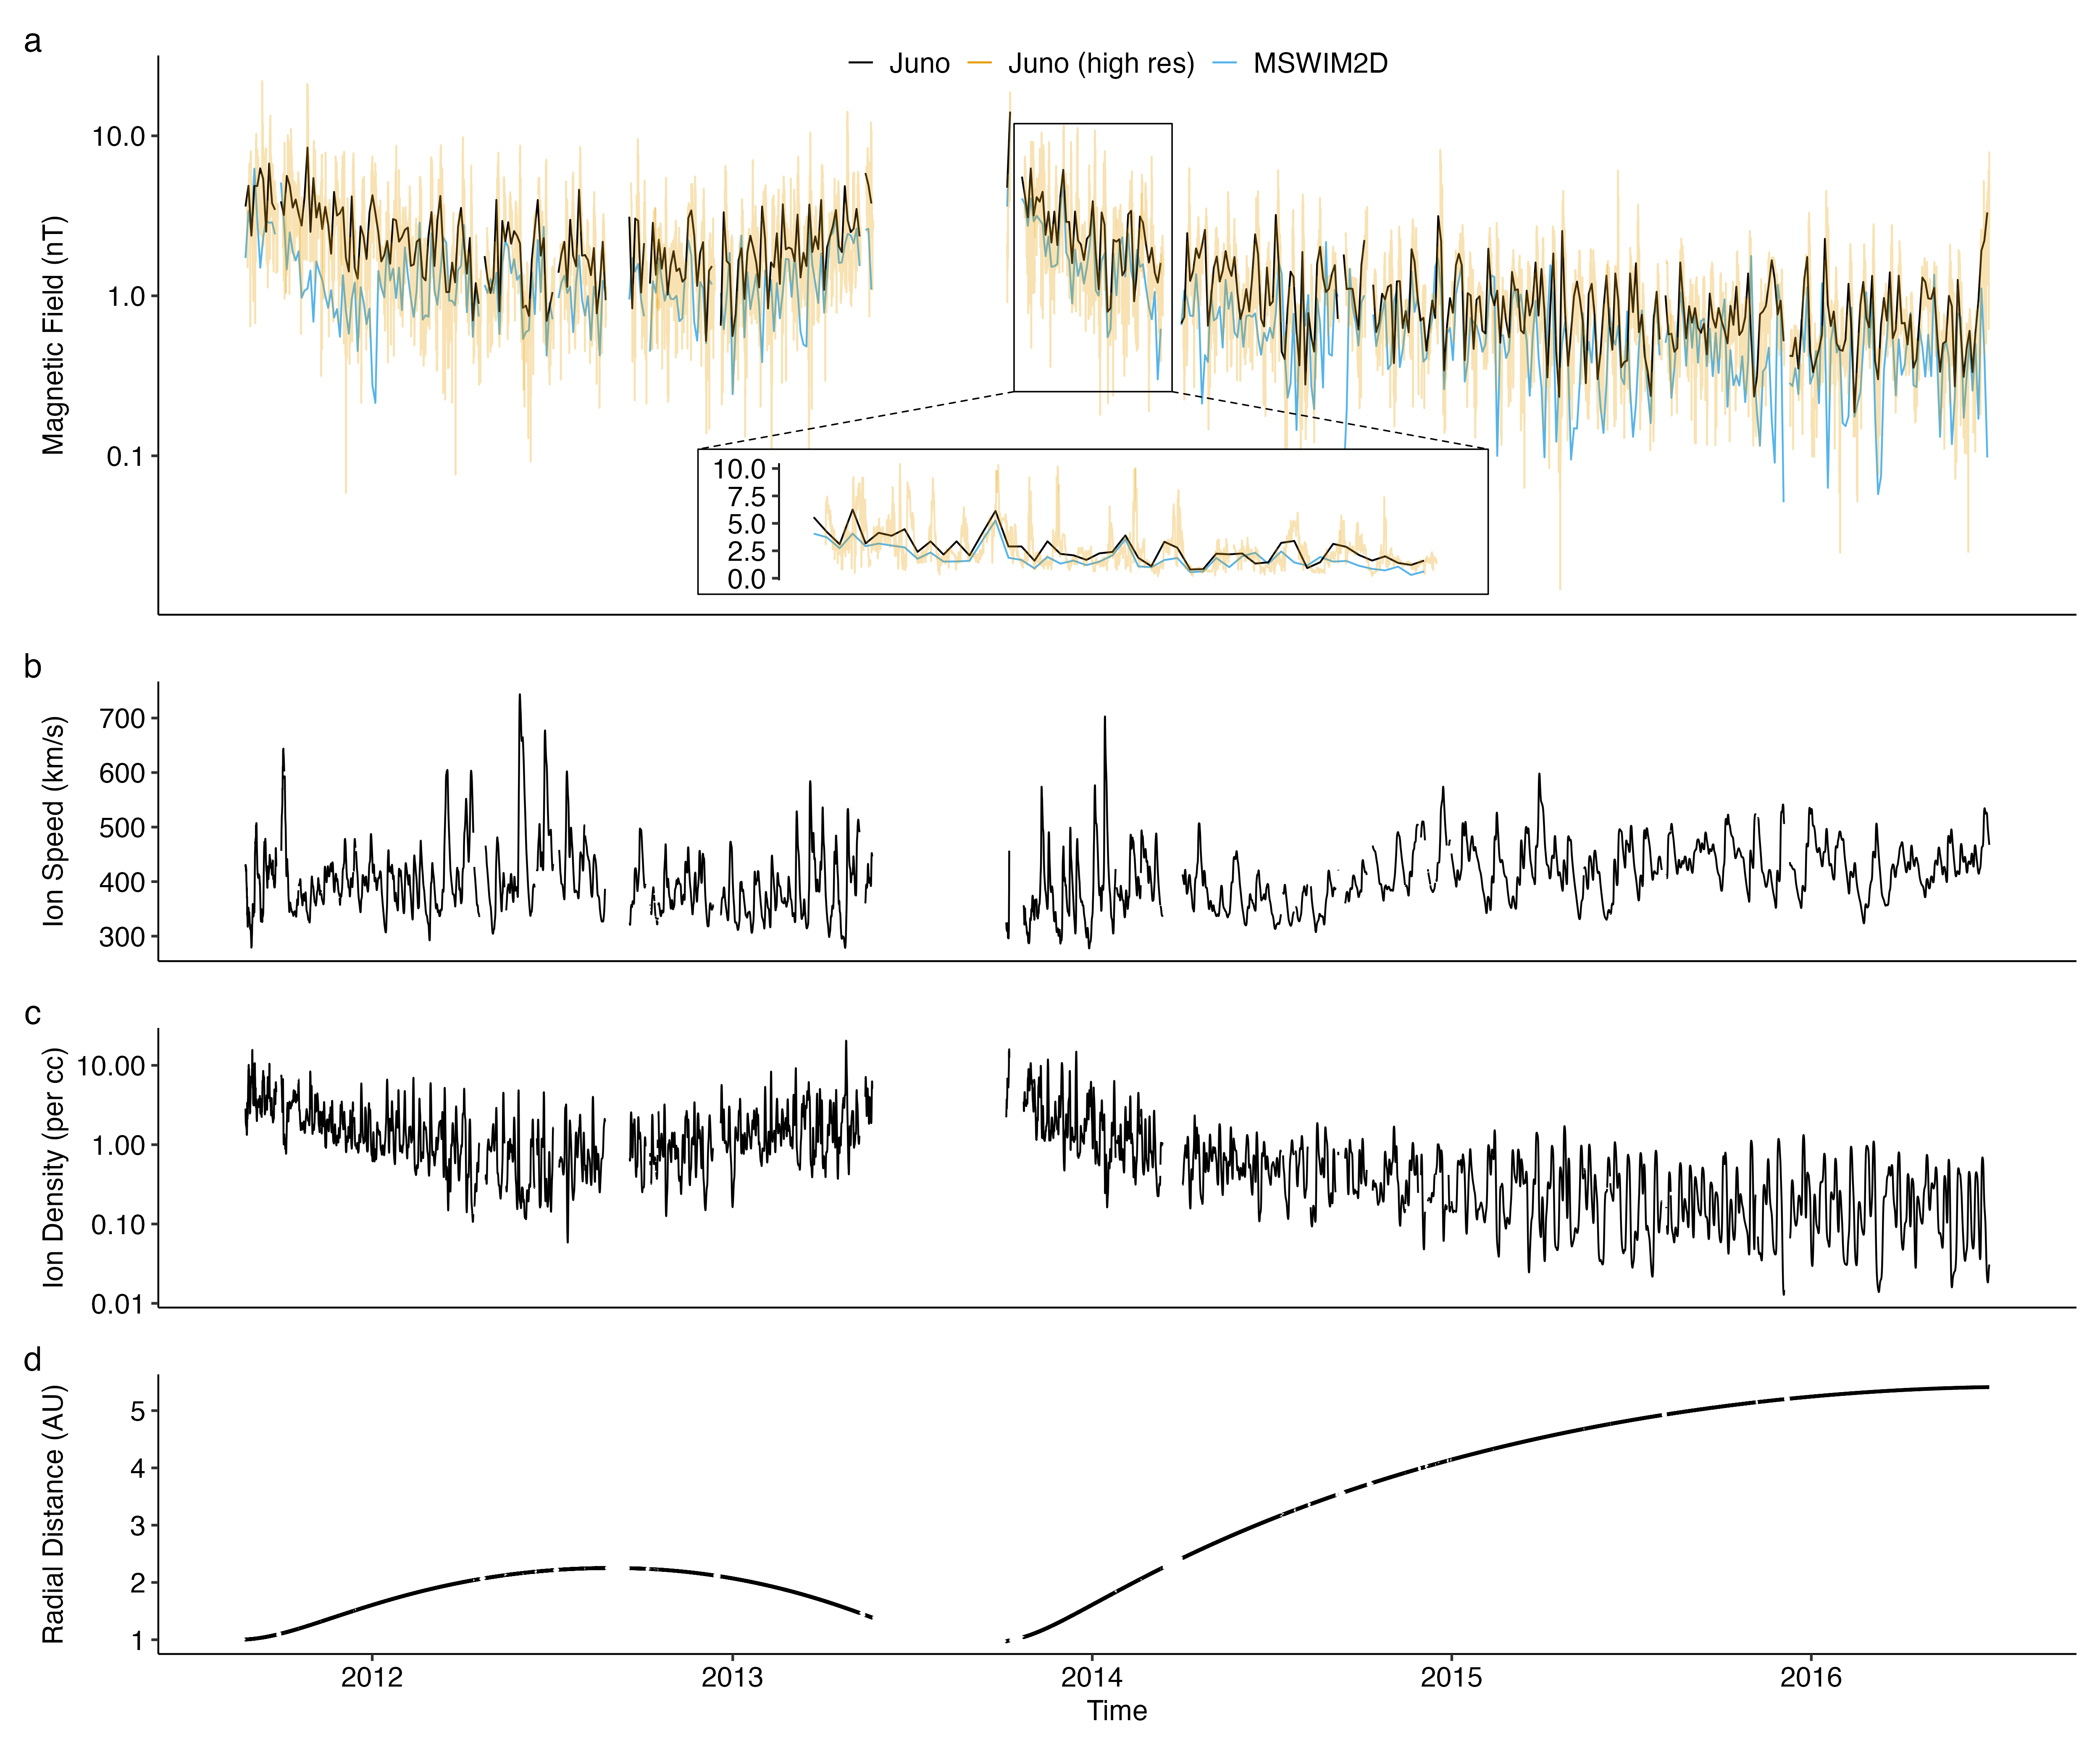
\includegraphics{figures/model/juno_model_validation_full.png}

}

\caption{\label{fig-model}\textbf{a,} Magnetic field magnitude from MSWIM2D and Juno. \textbf{b-c,} Plasma speed and density from MSWIM2D model. \textbf{d,} Juno radial distance from the Sun.}

\end{figure}%

\begin{figure}

\centering{

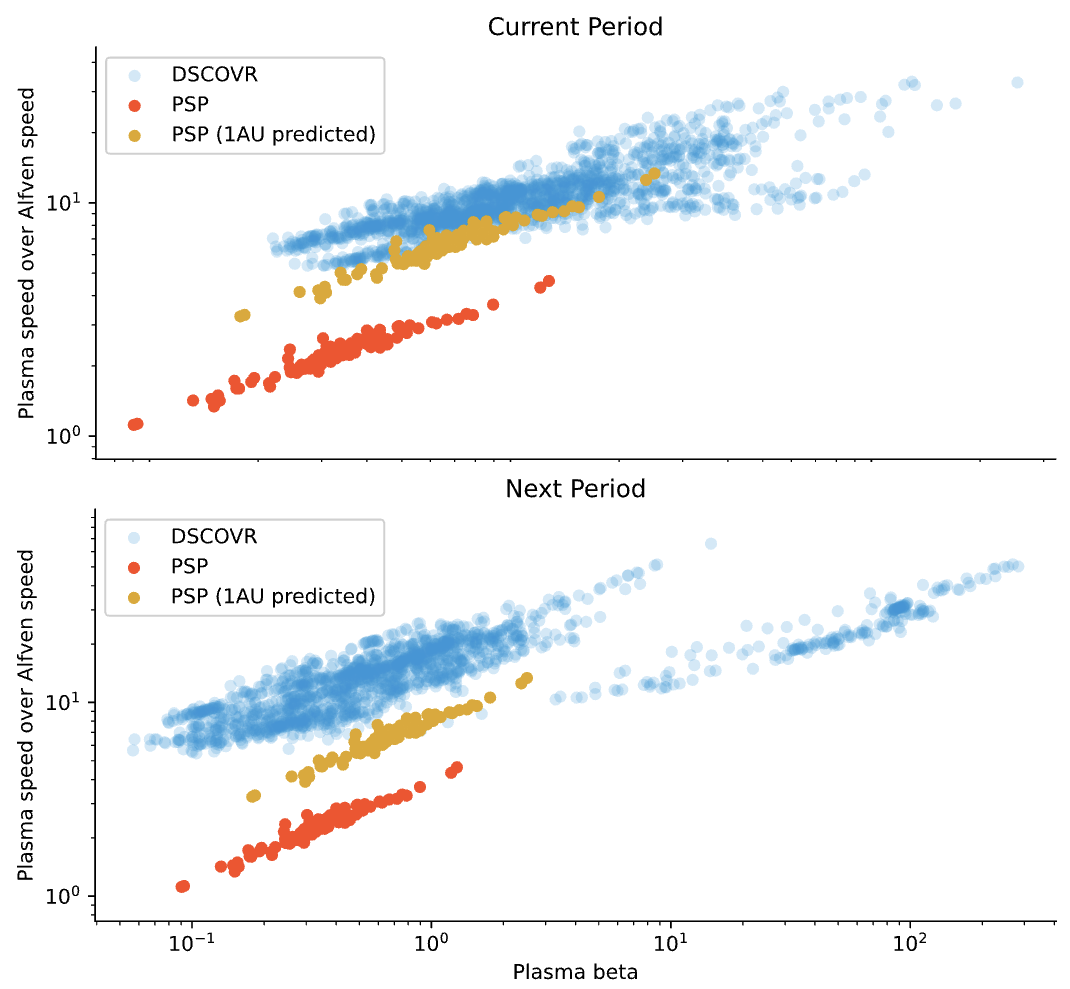
\includegraphics{figures/psp_properties_evolution.png}

}

\caption{\label{fig-evolution}Plasma properties (plasma beta versus plasma speed normalized by Alfven speed) measured by PSP projected to the ACE location using the statistical plasma expansion model. Top panel shows the data from the candidate alignment period (2019-04-06 to 2019-04-07) and the bottom panel shows the data after the alignment period.}

\end{figure}%

\newpage{}




\bibliography{files/Anton.addon.bib,files/Anton.full.bib,files/research.bib}


\end{document}
